\chapter{Extragalactic}

% -----------------------------
% -------- C G M --------------
% -----------------------------







\section{Circumgalactic Medium (CGM)}
\cite{2023VasilievEvgenii} : The discovery and intensive study of absorptions from heavy elements (such as CIV, SiIV, NV, OVI) in the circumgalactic medium (CGM) in quasar absorption spectra (e. g. Prochaska et al. 2006; Simcoe et al. 2006; Prochaska et al. 2017),  have posed \textbf{stellar feed-back} as one of the most important physical factors that determine, along with gravity, the structure and evolution of galaxies.


\section{Color-Color diagram}

A "colour" is the difference between two magnitudes, usually shorter minus longer wavelength, such that a positive colour means "redder". AGN can be identified using WISE colours. For example, Stern 2012 shows that the combined criteria W1 − W2 $\geq$ 0.8 and W2 $\leq$ 15 robustly identify an extremely robust, highly complete AGN sample. 

\begin{figure}
    \centering
    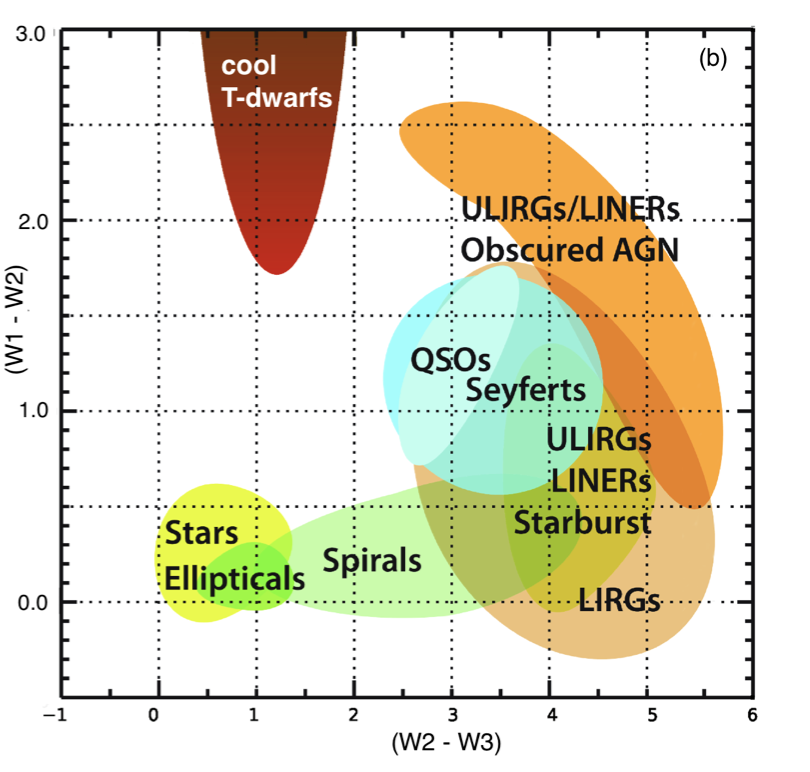
\includegraphics{Notes_Images/wise_color_color.png}
    \caption{W1, W2, and W3 stand for WISE magnitudes at 3.4, 4.6 and 12 $\mu$m, respectively. Based on the position of the galaxies on this plot, we can tell if they are star-forming spirals, cool stars or AGN. This plot is taken from Wright et al. 2010.  }
    \label{fig:enter-label}
\end{figure}


\section{Galactic Wind}

Galactic wind, a large-scale gas outflow from star formation in galactic discs, is thought to be driven by energy injection from young stars and supernovae in starburst events with a surface SFR exceeding a certain critical value. 
 The threshold for galactic winds driven by central starbursts is estimated at $ \varepsilon  \sim $ 10 erg cm $^{−2}$ s $^{−1}$ (Lehnert \& Heckman 1996a; Heckman 2000),  and for disc-halo circulation in edge-on galaxies $\varepsilon \sim$  10$^−3$ − 10$^−4$ erg cm$^{−2}$ s$^{−1}$ (Dahlem et al. 1995; Rossa et al. 2000; Dahlem et al. 2006). However, study of interrelations between the soft X-ray, UV, H$\alpha$, FIR and 1.4 GHz radio continuum emissions in a larger sample of 23 edge-on-galaxies led only to put a lower limit on the surface SN energy input rate $\varepsilon \geq$  10−3 erg cm$^{−2}$s$^{−1}$(Tüllmann et al. 2006).


\section{Galaxy Halos}

\cite{2023VasilievEvgenii} show that extended luminous haloes observed in edge-on galaxies (e.g., NGC891) can be maintained by disc-spread stellar clusters of smaller masses M$_∗$ $\sim < $  10 $^5$ M$_{\odot}$.



\section{Mid-infrared excess in galaxies}

Using a sample of $\sim$ 200 galaxies and active galactic nuclei (AGNs) from MOSDEF at 1.40< z< 2.61 with 24 $\mu$m detections (rest-frame 8 $\mu$m), \cite{2018Azadi} find that the Balmer line-derived SFRs or AGN activity are both not substantially higher in galaxies with mid-IR excess, alluding to the contribution of high mid-IR excess due to PAH contribution.



